\vspace*{-1cm}
\textbf{Overview:}
This project intends to increase the precision of the current ultrawide band indoor positioning system~\cite{decawave_product_brief}
in V207 using fusion with visual sensors.
The existing system determines the distances from ``tags'' to base stations using round trip
time of arrival.
While its accuracy is reasonably high (i.e.~it places the tag in generally the correct area),
its precision is low (i.e.~the perceived position is noisy and unpredictable within its error radius,
and it is slow to react to changes in position over time.
This can be seen in users' difficulty to play pong with the tags mounted to ping pong paddles:
the virtual paddle is difficult to control, moves without the users' input,
and sometimes reacts too slowly to users' movement,
such that they lose the game.

\begin{wrapfigure}{r}{6cm}
	%\begin{figure}
	\centering
	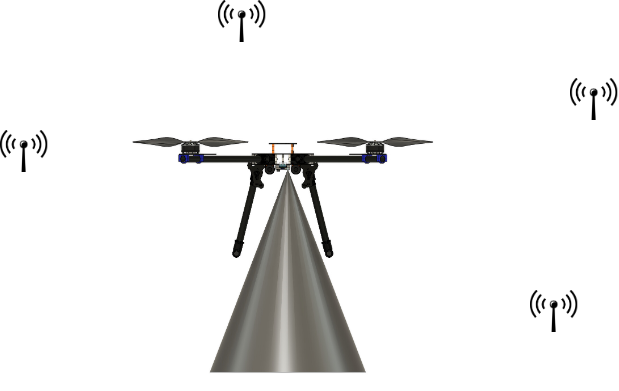
\includegraphics[width=5cm]{./images/sketch.png}
	\caption{The drone with visual sensors and radio beacons helping it to localize itself.}
\end{wrapfigure}

\textbf{Sensors:}
In this project I will augment the existing using sensors with which I will work in my future drone
projects -- namely an optical flow sensor and a depth camera.
The \emph{Ark Flow~\cite{arkflow} optical flow sensor} points vertically down
(with some error in just how vertical it is),
and measures pixel velocities in successive images in order to determine a velocity vector in 3
dimensions (clockwise/counter-clockwise, left/right, forwards/backwards).
It also has a LIDAR rangefinder which determines the height from the ground
(and can therefore derive vertical velocity).
This sensor may be inaccurate because the self-similarity of the floor may make it difficult
for it to determine pixel velocities correctly.
The second visual sensor will be a forward-facing \emph{Intel RealSense D455 depth camera},
which uses stereo vision (and in particular disparity) to determine distances to objects
in the environment.
Some extra processing/development will be required to identify and track salient obstacles in the
depth data, and these can be output directly as a list of relative positions to landmarks,
or translated into a velocity of the drone itself.
Further (optional) sensors include the inertial measurement units
of the depth camera and the flight controller.

\textbf{Data Processing}
The data will be collected in a time-synchronized stream as it is pushed on a cart around V207.
They will be timestamped when the system arrives at each of $n: 10 \leq n \leq 50$ points
whose ground-truth location is known by physically measuring it and then marking it on the ground.
Then, the data can be divided into subsets of sensors, in order to model and evaluate many different
systems simultaneously.
The data for each system will be fused using a Kalman filter.
The overall hope is that the system will mimick the functionality of
e.g.~an inertial measurement unit that is estimating its heading
from both a magnetometer (for long-term measurements in an absolute coordinate system),
and a gyroscope (for short-term measurements of angular velocity that can be integrated into a \emph{change} in position).

\textbf{Evaluation:}
The systems will be evaluated on their ability to accurately predict the positions of the drone
at each of the $n$ timestamps.
As such, the system will calculate the error distance from the drone's estimated position to each of the
ground-truth points.
I will also check the error distance as a function of time to see if the added sensors introduce
time-based positional drift that is not overcome by the ultrawide band system and Kalman filter.


